% \chapter{Bibliographic Survey}
\chapter{Studiu bibliografic}
\label{cap:studiu-bibliografic}
În acest capitol se face o prezentare a stagiului în care este domeniul; se detaliază cele mai bune sisteme de detecția obiectelor și segmentarea imaginilor de ultima oră prin informații căpătate din articole și cărți.\newline
Va fi vorbă despre viziunea artificială, rețelele neurale (mai ales architecturile folosite în procesarea imaginilor). Temele detecției obiectelor și segmentării semantice a imaginilor vor fi detaliate, prezentând caracteristicile specifice sistemelor inteligente capabile de a executa aceste sarcini.Dar mai întâi o imagine de ansamblu...\newline
\section{Imaginea de ansamblu}
De multe ori este o confuzie când vorbim despre conceptele de clasificarea imaginilor, detecția obiectelor și segmentarea semantică a imaginilor. După cum se vede în figura \ref{fig:class_detect_semgent} Toți trei fac parte din tematica înțelegerii unei imagini existând suprapuneri între aceștia, dar bineînțeles vorbim despre trei procese care diferă atât prin rezultatele executării cât și prin complexitatea algoritmilor care pot să le realizeze.\newline
Clasificarea imaginilor este procesul prin care după cum zice și numele, este procesul prin care obiectul fotografiat este înscrisă într-o categorie de obiecte (primind o imagine, sistemul trebuie să decidă clasa căreia aparține obiectul e.g. un câine sau o pisică).\newline
Detecția obiectelor pe de altă parte este procesul prin care identificăm locația a mai multor obiecte într-o imagine (sau numărarea instanțelor de un anumit tip de obiect într-o imagine). Majoritatea algoritmilor de detecția obiectelor (precum și algoritmul folosit în această lucrare) funcționează în următorul fel:
\begin{enumerate}
	\item un model sau un algoritm este folosit pentru generarea unei multitudini de regiuni de interest. Regiunile acoperă toată imaginea iar caracteristica lor comună este șansa ridicata de a fi bounding box pentru un obiect
	\item în pasul doi se extrag trăsături specifice din regiunile generate la pasul anterior. Se face o evaluare a trăsăturilor extrase și sistemul determină dacă regiunea respectivă conține un obiect, și dacă da, atunci ce fel de obiect (ce categorie). Acest pas este o componentă de clasificare a imaginilor
	\item ultimul pas este o post procesare, regiunile cu suprapuneri fiind combinate pentru alcătuirea unui bounding box
\end{enumerate}
Segmentarea semantică a unei imagini este procesul prin care imaginea digitală se partiționează în mai multi segmenți (seturi de pixeli cunoscute ca superpixeli). Scopul segmentării semantice este aceea de a simplifica și/sau de a schimba reprezentarea unei imagini pentru o înțelegere și analizare mai simplă. Segmentarea semantică este adesea folosită pentru localizarea obiectelor și a conturilor în imagini. Mai precis, segmentarea semantică a unei imagini este procesul prin care pentru fiecare pixel în asignăm o etichetă, astfel încât pixelii care împărtășesc aceeași etichetă, împărtășesc caracteristici definite (e.g. aparțin aceluiași obiect).
%image presenting image classification, detection and segmentation
\begin{figure}[h!]
    	\centering
	\captionsetup{justification=centering, margin=2cm}
	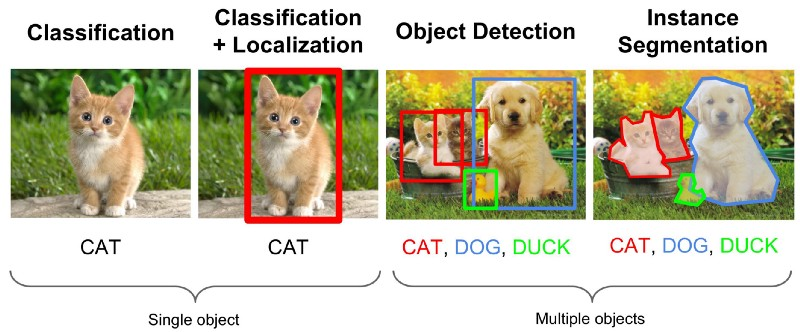
\includegraphics[width=0.9\textwidth]{figures/class_detect_segment.jpeg}
	\caption{Clasificare de imagine, localizare, detecție de obiecte, segmentare semantică \cite{class_detect_segment}}
	\label{fig:class_detect_semgent}
\end{figure}
\section{Domeniile din care face parte această lucarare}
\subsection{Viziunea Artificială}
Viziunea artificială este un domeniu interdisciplinar care se ocupă cu metode cu ajutorul cărora calculatoarele pot să câstige o întelegere la un nivel ridicat și abstract ale imaginilor digitale. Scopul este automatizarea proceselor de care sistemul vizual human este capabil.\newline
Problemele în acest domeniu se pot încadra în mai multe categorii cum ar fi obținerea, procesarea, analiza și întelegerea imaginilor digitale. \textit{Înțelegerea} în acest context înseamnă transformarea imaginilor vizuale în descrieri, care la rândul lor pot fi folosite în alte procese (e.g. luarea deciziilor). După \cite{Szeliski10computervision} viziunea artificială este folosită în următoarele domenii:
\begin{itemize}
	\item controlul proceselor, inspecție automatică
	\item navigare
	\item probleme de clasificare și organizare
	\item detectare de evenimente
	\item recunoaștere de obiecte, identificare (e.g. persounei după amprentă sau față, etc.), detectare (e.g. verificarea prezenței unui obiect pe o imagine)
	\item analiza mișcărilor, reconstruirea scenelor, restorarea imaginilor, etc.
\end{itemize}
\subsubsection{Metode uzuale în domeniul viziunii artificiale}
În \cite{M82computervision} Kusuma Kumari B. M. face o prezentare generală a metodelor des folosite în domeniul viziunii artificiale și procesarea imaginilor.\newline
După ce am obținut o imagine digitală, urmează pasul de \textbf{pre-procesare}. În acest pas putem aplica operații de re-sampling, intensificarea sau micșorarea contrastului, operații pentru a reduce zgomotul din imagine, transformări de culoare (binarizare, grayscale, etc.).\newline
Odată ce imaginea atinge o calitate anume (și putem să avem încredere că algoritmii următori pot să prelucreze imaginea) urmează de obicei pasul de \textbf{extragerea trăsăturilor}. Imaginea este scanată pentru trăsături specifice (astea aflându-se la o granularitate mare sau mică) care împreună definesc un obiect complex. De obicei cautăm linii, muchii, colțuri, puncte, cercuri, creste, etc.\newline
Am ajuns la pasul în care folosind trăsăturile extrase la pasul anterior facem o \textbf{procesare} la nivel înalt. Deja trebuie să lucrăm numai cu trăsăturile extrase, aceasta fiind o mare îmbunătățire față de situația ipotetică în care ar trebui să lucrăm cu imaginea digitală de intrare. Pe baza trasăturilor extrase putem să executăm recunoașteri de obiecte, sau să aplicăm alți algoritmi pe multitudinea trăsăturilor (de exemplu pentru construirea unei imagini noi).\newline
În anumite cazuri mai este un pas, și anume \textbf{luarea deciziilor}. Aici pe baza tuturor pașilor anteriori programul ia o decizie, cu asta împlinind funcționalitatea completă.
\subsection{Rețele Neuronale}
În această secțiune o să fie prezentată ideea de bază a funcționării rețelelor neuronale cu ajutorul unor articole.\newline
Dorffner ș.a. în \cite{dorffner1996neural} prezintă funcționarea de bază a rețelelor neuronale; rețelele neuronale artificiale sunt inspirate de natură, acestea încercând să reproducă funcționarea rețelelor de neuroni din sistemul nervos al animalelor. O rețea neuronală artificială ca și cea "naturală" este construită din neuroni care alcătuiesc straturi de neuroni. Neuronii din două straturi consecutive sunt legate, legătura având o pondere: un număr care exprimă puterea legăturii dintre cei doi neuroni.\newline
În \cite{rojas1996backpropagation} Rojas ș.a. prezintă conceptul care stă la baza antrenării unei rețele neuronale: retropropagarea erorii. 	Acest algoritm pornește de la un \textit{set de date de antrenare} format din perechi intrare - ieșire dorită. Ponderele rețelei se inițializează cu valori aleatorii, alese de obicei din intervalul (-1, 1).\newline
Algoritmul (în cea mai simplă formă a ei) are două stagii:
\begin{enumerate}
	\item rețeaua neuronală primește o intrare din setul de antrenare. Folosind valorile curente ale ponderilor se face propagarea înainte a informației de intrare, calculându-se ieșirea reală furnizată de rețea
	\item ieșirea reală se compară cu valoarea dorită corespunzătoare setului de antrenare si eroarea calculată astfel se propagă înapoi în rețea - de la stratul de ieșire, spre stratul de intrare - pentru modificarea ponderilor.
\end{enumerate}
În \cite{aima} autorii specifică caracteristicile definitive a unei rețele neuronale artificiale, astea fiind:
\begin{itemize}
	\item architectura rețelei este definită de mai multe aspecte: numărul straturilor de neuroni, numărul neuronilor pe fiecare strat, ponderile rețelei, etc.
	\item regula de învățare (learning rule) este mechanismul responsabil pentru ajustarea ponderilor în iterațiile învățării. Alegerea aceste reguli poate diferenția între eșec și succes
	\item regula de activare a unui neuron: ce se întâmplă internal în fiecare neuron? Cum sunt intrările lui prelucrate pentru a obține ieșirea? Regula de activare este descrisă de funcția de activare.
\end{itemize}
\subsection{Rețele neuronale convoluționale}
Pal, Nikhil R and Pal și Sankar K în \cite{pal1993review} prezintă că dintre technicile de segmentarea imaginilor, rețelele neuronale convoluționale întrec celelalte abordări cu o margine semnificativă.\newline
Rețelele neuronale convoluționale sunt foarte similare cu rețelele neuronale profunde clasice: sunt alcătuite din neuroni care au ponderi pe care pot să le învețe. Fiecare neuron are intrări, aplică funcția de activare și propagă mai departe activarea produsă.\newline
Deci ce se schimbă? Architecturile convoluționale se bazează pe asumpția explicită, că intrările sunt \textbf{imagini}. Această asumpție ne împuternicesc să facem o architectură mai avantajoasă. Astfel propagarea înainte devine mai eficientă iar costurile de antrenare se micșorează grozav.


Documentarea bibliografică are ca obiectiv fixarea referențialului în care se situează tema, prezentarea susrselor bibliografice utilizate și a cercetărilor similare și raportarea abordării din lucrare la acestea.

Referințele bibliografice se vor face pentru fiecare carte, articol sau material folosit pentru elaborarea lucrării de licență. 

Reprezintă cca. 10--15\% din lucrare.


% \section{Related Work}
\section{Abordări similare}

Comparați abordarea voastră cu cele ale altor soluții: ce e asemănător, ce e diferit (și, de preferat, mai bun). 

Citarea referințelor se face ca în exemplele \ref{subsec:s10} din Bibliografie. 
Vezi citările următoare.

În articolul \cite{Antoniou04} autorul descrie configurația tehnică a unei "honeynet" și prezintă câteva atacuri de actualitate asupra honeynet, precum și o serie de recomandări pentru securizarea sistemelor conectate la rețele de calculatoare.

% În capitolul 4 al [], referitor la valoare honeypots, Spitzner prezintă avantajele și dezavantajele acestora.

În articolul on-line \cite{electronic-citation} găsim detalii interesante despre \dots.


% \section{Technologies and Methods}
\section{Tehnici/Tehnologii/Surse folosite}

Sursele de documentare referitoare la metodele, tehnologiile, ideile folosite. 



